\documentclass[11pt,a4paper]{article}

\usepackage[margin=25mm]{geometry}
\usepackage{amsmath,amssymb}
\usepackage{graphicx}
\usepackage{booktabs}
\usepackage{siunitx}
\usepackage{tikz}
\usetikzlibrary{arrows.meta,positioning,fit}
\usepackage[numbers]{natbib}
\usepackage[hidelinks]{hyperref}

% Written by make_figures.jl
\newcommand{\MaxHeading}{40.0}
\newcommand{\Period}{15.0}
\newcommand{\SimTime}{20.0}
\newcommand{\SettleTime}{5.0}
\newcommand{\NumSections}{10}
\newcommand{\NumPanels}{72}
\newcommand{\CaseRows}{
\code{AeroDirect} & 50 & 1 & 1.8 & 0 & 22.4 & 0 & -- & -- & -- & -- \\
\code{AeroDirect} & 10 & 1 & 3.5 & 0 & 134.4 & 0 & -- & -- & -- & -- \\
\code{AeroDirect} & 2 & 1 & 3.4 & 0 & 2.2 & 61 & -- & -- & -- & -- \\
\code{AeroDirect} & 10 & 5 & 2.4 & 17 & 62.1 & 1 & -- & -- & -- & -- \\
\code{ContinuousAero} & 50 & 1 & 4.0 & 0 & 2.1 & 3 & -- & -- & -- & -- \\
\code{ContinuousAero} & 10 & 1 & 4.0 & 0 & 2.0 & 16 & -- & -- & -- & -- \\
\code{ContinuousAero} & 10 & 5 & 4.0 & 0 & 1.8 & 4 & -- & -- & -- & -- \\
\code{AeroPressure} & 50 & 1 & 20.0 & 0 & 2.1 & 13 & 0.86 & 0.06 & 20.0 & 0.044 \\
\code{AeroPressure} & 10 & 1 & 20.0 & 2 & 2.1 & 71 & 0.85 & 0.02 & 19.0 & 0.040 \\
\code{AeroPressure+live} & 50 & 1 & 1.2 & 21 & 1.7 & 42 & -- & -- & -- & -- \\
\code{AeroPressure+live} & 10 & 1 & 1.5 & 4 & 5.0 & 50 & -- & -- & -- & -- \\
}


\newcommand{\code}[1]{\texttt{#1}}
\newcommand{\vect}[1]{\boldsymbol{#1}}

\title{Four ways to couple a vortex-step aerodynamic model to a flexible kite:\\
a comparison on the TU~Delft V3}
\author{SymbolicAWEModels.jl contributors}
\date{\today}

\begin{document}
\maketitle

\begin{abstract}
A flexible kite is simulated by coupling a structural model with many degrees of
freedom to an aerodynamic model that is too expensive to solve at every evaluation of
the equations of motion. SymbolicAWEModels.jl offers four ways to make that coupling
with the Vortex Step Method (VSM): \code{AeroDirect} holds the solved panel forces
constant between solves; \code{ContinuousAero} holds only the induced velocity and
re-evaluates every panel force from the live wing state; \code{AeroPressure} does the
same and places each panel force on the structure through the airfoil pressure
distribution; and \code{AeroPressure} with live polars also regenerates each panel's
polar and pressure distribution from its deformed shape with NeuralFoil. We fly the
Timoshenko-beam model of the TU~Delft V3 kite, built with V3Kite.jl, under all four
couplings through the same heading manoeuvre and compare their stability, cost, load
placement and sensitivity to deformation. \ResultAbstract
\end{abstract}

\section{Introduction}

The leading-edge inflatable (LEI) kites used for airborne wind energy deform
substantially in flight: the canopy billows, the struts bend and the whole wing twists
when it is steered through its bridle. An aero-structural model of such a kite pairs a
structural model, here a lattice of Timoshenko beams, bridle lines and point masses,
with an aerodynamic model that turns the deformed shape and the apparent wind into
loads. A lifting-line model with 2D section polars, the Vortex Step Method
(VSM)~\citep{cayon2023vsm,vortexstepmethod}, is accurate enough for a curved LEI wing
and cheap enough to run inside a dynamic simulation~\citep{poland2023}, but solving its
nonlinear circulation problem at every evaluation of the structural right-hand side
(RHS) is still far too expensive for an implicit time integrator that evaluates the RHS
and its Jacobian many times per step.

The coupling therefore always freezes \emph{something} between VSM solves. What is
frozen decides three properties of the simulation:
\begin{enumerate}
  \item whether the aerodynamic forces respond to the wing's motion between solves,
    which is what supplies aerodynamic damping to fast structural modes;
  \item where on the structure each panel force is applied;
  \item which deformations of the wing the section polars can see.
\end{enumerate}
SymbolicAWEModels.jl~\citep{symbolicawemodels} implements four couplings that make
different choices, selected per wing with the \code{aero\_mode} argument of
\code{load\_sys\_struct\_from\_yaml}. This paper describes them in a common notation,
flies each on the same kite and manoeuvre, and states what each one is for.

\section{Aero-structural model}

\subsection{The V3 kite}

The TU~Delft V3 is a \SI{25}{m^2} LEI kite with a well documented geometry. We use the
Timoshenko-beam model of V3Kite.jl~\citep{v3kite}
(\code{system\_beam.yaml}): the leading edge and the struts are inflated beams joined
at ten structural stations, each carrying a leading-edge point, a trailing-edge point
and eleven chordwise control points on the canopy; the bridle is a network of spring
segments and pulleys down to a kite control unit and a braked winch holding
\SI{250}{m} of tether. The aerodynamic geometry has \NumSections{} sections sliced
from the V3 surface mesh, with NeuralFoil~\citep{neuralfoil} polars and surface
pressure tables for every section, and is refined into \NumPanels{} VSM panels.

\subsection{Common aerodynamic core}

Every coupling starts from the same VSM solve. Given the panel geometry and the
apparent wind $\vect{v}_{a,i}$ at each panel $i$, the solver finds the bound
circulation $\Gamma_i$ that makes the lift of each panel consistent with its section
polar at its effective angle of attack. From the converged solution follow the induced
velocity $\vect{v}_{\mathrm{ind},i}$ at each panel's control point and the panel force
\begin{equation}
  \vect{F}_i = q_i\, c_i\, b_i \left( C_{L}(\alpha_i)\,\hat{\vect{l}}_i
             + C_{D}(\alpha_i)\,\hat{\vect{d}}_i \right),
  \qquad
  q_i = \tfrac{1}{2}\rho \left| \vect{v}_{a,i} + \vect{v}_{\mathrm{ind},i} \right|^2 ,
  \label{eq:panel-force}
\end{equation}
with chord $c_i$, span $b_i$, and lift and drag directions $\hat{\vect{l}}_i$,
$\hat{\vect{d}}_i$ normal and parallel to the effective inflow. The angle of attack
$\alpha_i$ is measured in the panel's own chord frame, which is reconstructed from the
structural points that bound it. A VSM solve runs every \code{vsm\_interval} time steps
of the structural integrator; the couplings differ in what they keep from it.

\subsection{The four couplings}

Figure~\ref{fig:coupling} shows the data flow of each coupling.

\begin{figure}[t]
\centering
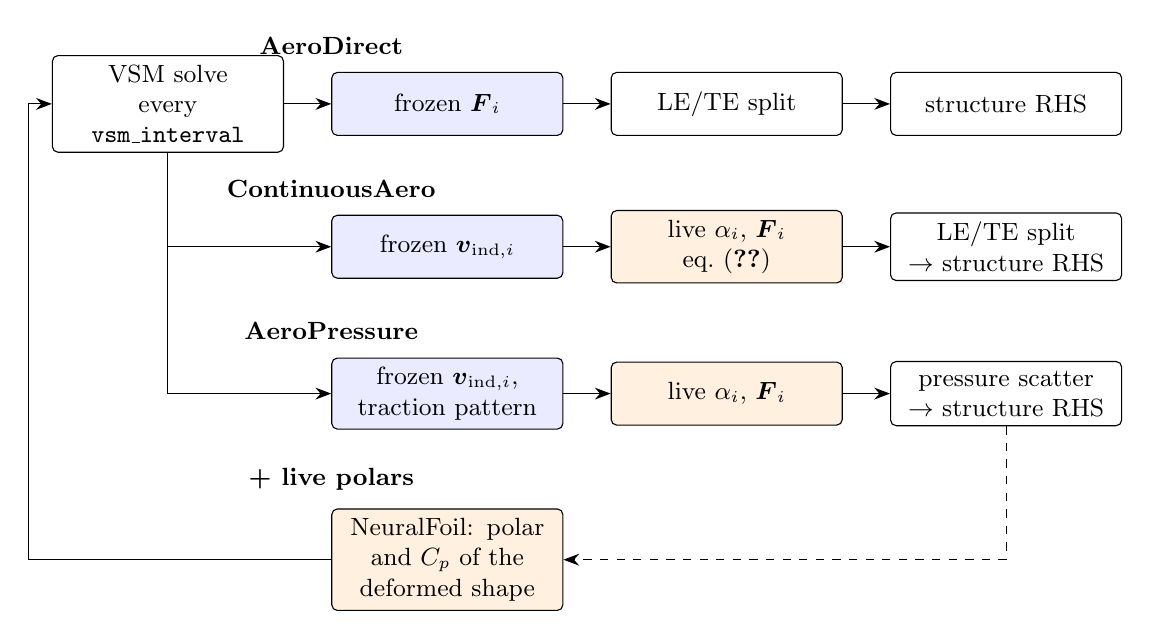
\begin{tikzpicture}[
  node distance=4mm and 6mm,
  box/.style={draw, rounded corners=2pt, align=center, font=\small,
              minimum height=8mm, text width=27mm},
  frozen/.style={box, fill=blue!8},
  live/.style={box, fill=orange!12},
  lab/.style={font=\small\bfseries, anchor=west},
  arr/.style={-{Stealth[length=2mm]}},
]
\node[box] (vsm) {VSM solve\\ every \code{vsm\_interval}};
\node[frozen, right=of vsm] (df) {frozen $\vect{F}_i$};
\node[box, right=of df] (dle) {LE/TE split};
\node[box, right=of dle] (s1) {structure RHS};
\node[lab, above=1mm of df.north west] {AeroDirect};
\draw[arr] (vsm) -- (df); \draw[arr] (df) -- (dle); \draw[arr] (dle) -- (s1);

\node[frozen, below=10mm of df] (cv) {frozen $\vect{v}_{\mathrm{ind},i}$};
\node[live, right=of cv] (cf) {live $\alpha_i$, $\vect{F}_i$\\ eq.~\eqref{eq:panel-force}};
\node[box, right=of cf] (s2) {LE/TE split\\ $\to$ structure RHS};
\node[lab, above=1mm of cv.north west] {ContinuousAero};
\draw[arr] (vsm) |- (cv); \draw[arr] (cv) -- (cf); \draw[arr] (cf) -- (s2);

\node[frozen, below=10mm of cv] (pv) {frozen $\vect{v}_{\mathrm{ind},i}$,\\ traction pattern};
\node[live, right=of pv] (pf) {live $\alpha_i$, $\vect{F}_i$};
\node[box, right=of pf] (s3) {pressure scatter\\ $\to$ structure RHS};
\node[lab, above=1mm of pv.north west] {AeroPressure};
\draw[arr] (vsm) |- (pv); \draw[arr] (pv) -- (pf); \draw[arr] (pf) -- (s3);

\node[live, below=10mm of pv] (lp) {NeuralFoil: polar\\ and $C_p$ of the\\ deformed shape};
\node[lab, above=1mm of lp.north west] {+ live polars};
\draw[arr] (lp.west) -| ([xshift=-3mm]vsm.south west) -- ([xshift=-3mm]vsm.north west |- vsm.west) -- (vsm.west);
\draw[arr, dashed] (s3.south) |- (lp.east);
\end{tikzpicture}
\caption{What each coupling freezes at a VSM solve (blue) and what it re-evaluates at
every RHS evaluation of the structural model (orange). Live polars add a NeuralFoil
evaluation of the deformed sections before each solve.}
\label{fig:coupling}
\end{figure}

\paragraph{AeroDirect.}
The panel forces of the last solve are distributed to the structure and held constant
until the next one,
\begin{equation}
  \vect{F}_j(t) = \vect{F}_j(t_k), \qquad t_k \le t < t_{k+1},
\end{equation}
a zero-order hold. Each panel's force and moment are split between the leading- and
trailing-edge points of its section such that both are preserved. The RHS reads the
point forces as parameters, so the aerodynamics adds nothing to the cost of an RHS
evaluation or to the Jacobian. It is the simplest coupling and the only one that
supports every VSM wing type, but it is a loosely coupled, explicit partitioned
scheme~\citep{farhat2006}: within a step the structure moves under forces that do not
know it moved, and the structural Jacobian contains no aerodynamic damping.

\paragraph{ContinuousAero.}
Only the circulation solve is frozen. At each solve the induced velocity of every
refined panel is stored, and every RHS evaluation rebuilds each panel's chord frame from
the live structural points, forms the inflow
$\vect{v}_{a,i}(\vect{x},\dot{\vect{x}}) + \vect{v}_{\mathrm{ind},i}$, and evaluates
eq.~\eqref{eq:panel-force} symbolically with the section polars at the resulting
$\alpha_i$. The force on each panel is scattered onto its two bounding sections as
$0.75\,\vect{F}_i + \vect{C}_i$ at the leading edge and $0.25\,\vect{F}_i - \vect{C}_i$
at the trailing edge, where the couple $\vect{C}_i$ carries the pitching moment. Because
$\partial\vect{F}/\partial\dot{\vect{x}}$ now enters the Jacobian, the implicit
integrator sees the aerodynamic damping of every mode that changes the angle of
attack, and a stale induced velocity costs far less than a stale force: the induced
velocity changes with the circulation distribution, which varies slowly compared with
the local inflow.

\paragraph{AeroPressure.}
The panel force is evaluated exactly as in \code{ContinuousAero}, but it is placed on
the structure through the airfoil's surface traction. At each solve the section's
pressure and skin-friction tables are evaluated at the panel's angle of attack, and each
contour node $k$ receives the traction
\begin{equation}
  \vect{t}_k = \left( -C_{p,k}\,\hat{\vect{n}}_k + c_{f,k}\,\hat{\vect{s}}_k \right)
               q\, A_k ,
\end{equation}
which is lofted onto the nearest structural points of the panel's station. Between
solves the traction pattern is frozen, and each point receives its frozen traction plus
an equal share of the difference between the live panel force and the frozen pattern's
net force, so the point forces always sum to the live total. VSM owns the magnitude,
the pressure distribution owns the placement. On a wing whose stations carry chordwise
points, such as the beam V3, this is the only coupling that loads the canopy between
the leading and trailing edge.

\paragraph{AeroPressure with live polars.}
The tabulated polars of the three couplings above belong to the undeformed sections, or
to a family of sections indexed by a single flap angle. With live polars every
station's chordwise control points are read as a deformation of its airfoil: their
offsets from the deformed chord line become an increment of the section's Kulfan
(CST) parameters~\citep{kulfan2008}, NeuralFoil is evaluated on a grid of angles of
attack around each panel's current $\alpha$, and the result becomes the panel's polar
for the next solve. After the solve, the pressure distribution is regenerated from the
same deformed shape. The polars therefore follow any chordwise deformation the
structure can express, not only a known flap or chord-fraction deformation, at the
price of a neural-network evaluation per solve whose accuracy is only as good as
NeuralFoil's for the deformed shape.

\section{Test case}

All cases start from the same settled state of the beam V3 at \SI{250}{m} tether length,
\SI{60}{\degree} elevation and \SI{20}{\percent} depower, with the winch braked. A
proportional heading controller (V3Kite's \code{heading\_settings\_beam.yaml}, gain
$K=1$, steering limited to \num{0.15}) tracks the setpoint
$\psi_{\mathrm{ref}}(t) = \SI{\MaxHeading}{\degree}\sin(2\pi t/\SI{\Period}{s})$
for \SI{\SimTime}{s}. The structure is integrated with the FBDF solver of V3Kite's
settings at a fixed output step $\Delta t$ of \SI{50}{ms} or \SI{10}{ms}. Each
coupling is flown at both steps with a VSM solve every step, and the two cheaper
couplings are also flown at \SI{10}{ms} with a solve every fifth step. A case stops
early when the integrator fails, the wing's geometry becomes invalid for the VSM,
more than \num{20} VSM solves fail to converge, or it has run for
\SI{20}{min} of wall time. The wall times are single-threaded, measured by the
simulation's own step timers on one core of a shared machine, and are comparable
between the cases only to within some ten percent.

\section{Results}

\begin{table}[t]
\centering
\small
\caption{The cases. $\Delta t$ is the output step, $n$ the steps between VSM solves,
$T$ the time flown before the case ended and $N_f$ the VSM solves that did not
converge. Cost is integration plus VSM time per simulated second, first step excluded,
and the share of it spent in the VSM
solves. The flight statistics are taken after \SI{\SettleTime}{s}: mean tether force
$\bar F_t$, RMS angle of attack above \SI{2}{Hz} $\tilde\alpha$, RMS heading error
$e_\psi$, and RMS mean wing-node speed above \SI{2}{Hz} $\tilde v$.}
\label{tab:cases}
\setlength{\tabcolsep}{4pt}
\begin{tabular}{lrrrrrrrrrr}
\toprule
coupling & $\Delta t$ & $n$ & $T$ & $N_f$ & cost & VSM & $\bar F_t$ & $\tilde\alpha$
  & $e_\psi$ & $\tilde v$ \\
 & [ms] & & [s] & & [s/s] & [\%] & [kN] & [°] & [°] & [m/s] \\
\midrule
\CaseRows
\bottomrule
\end{tabular}
\end{table}

RESULTS_TEXT

\section{Discussion}

DISCUSSION_TEXT

\section{Reproducing the results}

The paper lives in \code{papers/aero\_couplings} of the SymbolicAWEModels.jl
repository. \code{make\_aero\_geometry.jl} slices the V3 mesh and writes the NeuralFoil
section tables, \code{run\_simulations.jl} flies the cases and logs them, and
\code{make\_figures.jl} writes the figures and the numbers quoted here. The figures use
the plotting functions \code{plot\_station\_loads!}, \code{plot\_panel\_polar!} and
\code{plot\_panel\_pressure!} of the package's Makie extension.

\bibliographystyle{unsrtnat}
\bibliography{references}

\end{document}
